\documentclass[crop,tikz]{standalone}

\usepackage[locale=DE]{siunitx}
\usepackage{pgfplots}
\tikzset{>=latex}

\pgfplotsset{
  inverted/.style = {
    every axis legend/.append style={
      draw=white,
      fill=hardblack,
      text=white
    }
  }
}

\begin{document}
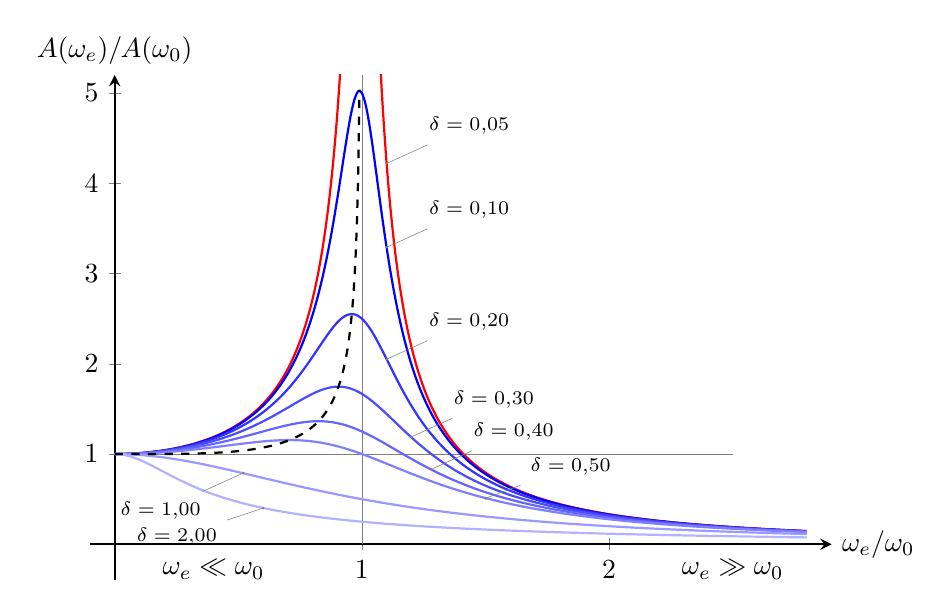
\begin{tikzpicture}[
      every pin/.style={
        font=\scriptsize,
        pin distance=3ex},
      small dot/.style={
        fill=gray,
        circle,
        scale=0.1}]
    \begin{axis}[
      thick,
      samples=100,
      axis y line=middle,
      axis x line=middle,
      xlabel style={at=(current axis.right of origin), anchor=west},
      ylabel style={at=(current axis.above origin), anchor=south},
      % labels
      % tick label style={font=\scriptsize},
      xlabel={$\omega_e/\omega_0$},
      ylabel={$A(\omega_e)/A(\omega_0)$},
      ytick={0,1,2,3,4,5},
      xtick={0,1,2,3},
      xticklabels={0,$1$,$2$,},
      % plot lines property
      no markers,
      cycle list={{black,solid}},
      % dominio 2D
      samples=200,
      smooth,
      domain=0:2.8,
      xmin=-0.1, xmax=2.9,
      ymin=-0.4, ymax=5.2,
      % canvas dimensions
      width=11cm, 
      height=8cm
      ]

      % horizontal help line
      \draw[help lines] (axis cs:0,1) -- (axis cs:2.5,1);
      % vertical help line
      \draw[help lines] (axis cs:1,0) -- (axis cs:1,5.2);

      % curves
      \addplot [color=red    , smooth, thick]{1/sqrt((1-x^2)^2+4*0.05^2*x^2)};
      \addplot [color=blue   , smooth, thick]{1/sqrt((1-x^2)^2+4*0.10^2*x^2)};
      \addplot [color=blue!80, smooth, thick]{1/sqrt((1-x^2)^2+4*0.20^2*x^2)};
      \addplot [color=blue!70, smooth, thick]{1/sqrt((1-x^2)^2+4*0.30^2*x^2)};
      \addplot [color=blue!60, smooth, thick]{1/sqrt((1-x^2)^2+4*0.40^2*x^2)};
      \addplot [color=blue!50, smooth, thick]{1/sqrt((1-x^2)^2+4*0.50^2*x^2)};
      \addplot [color=blue!40, smooth, thick]{1/sqrt((1-x^2)^2+4*1.00^2*x^2)};
      \addplot [color=blue!30, smooth, thick]{1/sqrt((1-x^2)^2+4*2.00^2*x^2)};

      % resonance
      \addplot[dashed,domain=0:0.99] {1/sqrt(1-x^4)};

      % pins
      \node[small dot,pin=30:{$\delta=\num{0,05}$}] at (axis cs:1.10,4.22) {};
      \node[small dot,pin=30:{$\delta=\num{0,10}$}] at (axis cs:1.10,3.29) {};
      \node[small dot,pin=30:{$\delta=\num{0,20}$}] at (axis cs:1.10,2.05) {};
      \node[small dot,pin=30:{$\delta=\num{0,30}$}] at (axis cs:1.20,1.19) {};
      \node[small dot,pin=30:{$\delta=\num{0,40}$}] at (axis cs:1.28,0.83) {};
      \node[small dot,pin=20:{$\delta=\num{0,50}$}] at (axis cs:1.50,0.51) {};
      \node[small dot,pin=210:{$\delta=\num{1,00}$}] at (axis cs:0.52,0.79) {};
      \node[small dot,pin=195:{$\delta=\num{2,00}$}] at (axis cs:0.60,0.40) {};
      \node[black] at (axis cs:0.4,-0.28) {$\omega_e\ll\omega_0$};
      \node[black] at (axis cs:2.5,-0.28) {$\omega_e\gg\omega_0$};
    \end{axis}
\end{tikzpicture}
\end{document}
